\documentclass{article}
\usepackage{graphicx,color}
\usepackage{times}

\begin{document}
\title{Manual: How To Use This Dissertation Template}
\author{by Svetlana Lockwood\\
  School of Electrical Engineering and Computer Science\\
  Washington State University\\
  \texttt{svetlana.lockwood@email.wsu.edu}}
\maketitle

\section{Why LaTeX{}?}\label{sl:why}
\subsection{Why, indeed?}
This dissertation LaTeX{} template provides a convenient form which you can fill in. All the formatting - the title, the fonts, the paragraphs, the spacings and alignments, the page numbering with all the escapes and re-starts, the sections and subsections numbering - in one word, {\em \uppercase{everything}} has been done for you! Isn't that wonderful?! What left for you is to fill in this form with {\em your} content.
\subsection{What are the benefits of using LaTeX{}?}\label{latex_benefit}
Short answer: many. And if you have never used LaTeX{} before, you'll have to spend a couple of hours to get started, but that will save tons of time ahead. 
\subsection{Specifications and last update}\label{last_update}
This manual explains how to use this template. It also contains a tutorial that primarily for those who have little or no experience with LaTeX{}. 

The dissertation template was made to specifically satisfy the requirements of the graduate school at Washington State University (WSU). In particular, it is pre-set to produce Ph.D. dissertations for a student of School of Electrical Engineering and Computer Science of WSU. However, these parameters can be easily changed as explained below. Citation style is set to APA-like, i.e., author name and year.

The last update of this template was done on \date{\today}. The author of this manual operates on a Windows computer. Therefore, all the remarks and software notices are for Windows-users.
\section{Tutorial: Quick start on LaTeX{}}\label{sl:quick_start}
If you have never used LaTeX{} before, I suggest looking for some web resource for an overview of LaTeX{} features. In-depth tutorials may be helpful further down the road. However, this tutorial will provide you with all necessary information to get you started quickly. 
\subsection{Background}\label{latex_background}
LaTeX{} is somewhat different than Word. The content and formatting are separated from each other. In that LaTeX{} reminds HTML with its CSS files, and if you have done some HTML, you will have to difficulties writing in LaTeX{}. Thus, once the formatting is done - and that has already been done for you - all is left is to write the text. Your usual mode of operation is:
\begin{enumerate} \itemsep1pt \parskip0pt \parsep0pt
  \item Write some text and save it.
  \item Build the document - as easy as to push a button.
  \item Preview your document and see if you are happy with it.
  \item Repeat until done.
\end{enumerate}
\subsection{Your very first step}\label{latex_1st_step}
Your very first step is to acquire software in which you are going to write your text. I highly recommend TeXstudio. TeXstudio provides a user-friendly interface. It has many useful features among which is also a spell-checker. Most valuable of it is - with TeXstudio you do not need to become a programmer to learn to write in LaTeX{}! TeXstudio is Windows-friendly. In fact, I'm using it right now for writing this text. 
\subsection{Your next step}\label{latex_2nd_step}
Your next step is to run a small pilot test to get yourself comfortable with your newly acquired TeXstudio. You are ready to create your first LaTeX{} document. Make a separate folder where you are going to save your first LaTeX{} document, open TeXstudio, start a new document and copy the following text into it:
\begin{verbatim}
\documentclass{article}
\begin{document}

\title{Here is My Beautiful Title}
\author{this is my name}
\maketitle

\section{Introduction}
Here is the text of my introduction.

\section{Main Text}
Here is the text of my main text.

\section{Conclusion}
And here's my conclusion. Good-bye!

\end{document}
\end{verbatim}
Now save your file in the designated folder and in TeXstudio press 'Build and View' button, Fig.~\ref{fig_build_view_btn}.
\begin{figure}[ht!]
    \centering
    
\includegraphics[width=0.5in]{btn_build.png}
    \caption{'Build and View' button.}
    \label{fig_build_view_btn}
\end{figure}
\begin{figure}[hb!]
    \makebox[\textwidth][c]{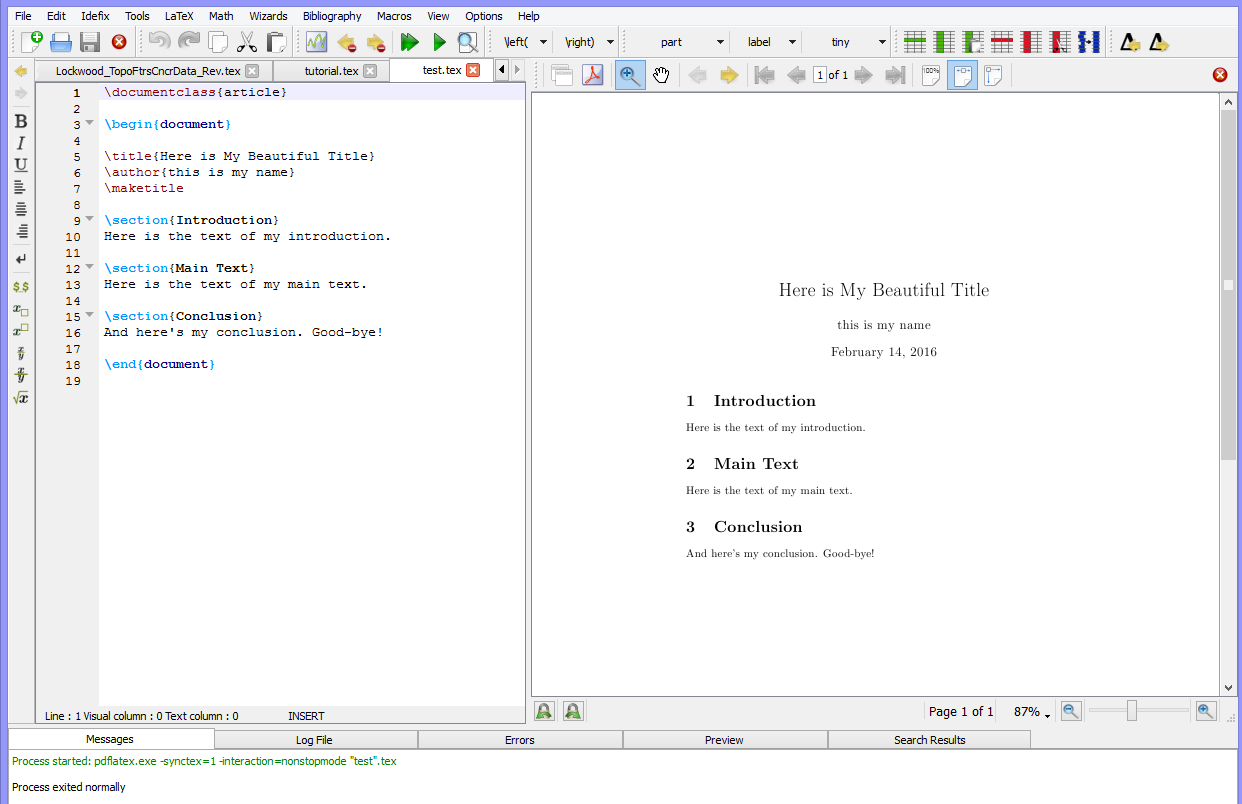
\includegraphics[width=1.4\textwidth]{result.png}}   
    \caption{Your first LaTeX{} document.}
    \label{fig_result}
\end{figure}
The build will most likely take a few seconds and at the bottom you'll see the compiler messages. Then a new window opens on the right to show you the results. Congratulations! You've just made your first LaTeX{} document! TeXstudio automatically creates a PDF file for you which you'll find the designated folder. It will have the same name as your \texttt{.tex} file. Now try to change some text, re-build it and see how your changes affect the document.

\subsection{A few important notes}\label{latex_notes}
In the text editor (left side of Figure~\ref{fig_result}) you noticed some text is colored. That's the assistance provided to you by TeXstudio - the coding commands are highlighted by the colors. Coding commands instruct the computer how to represent the text. If you try to change them, you'll probably get an error. The text you can change is black.

Just as you do in Word, do not press Enter at the end of each line when typing a paragraph. Paragraph wrapping will occur automatically. Press Enter twice (insert an empty line) to start a new paragraph.

Do not worry if you do not know all LaTeX{} commands. I do not know them either. The beauty of using this template is that you do not have to know any commands because the whole dissertation has already been pre-formatted for you. All you have to do is to provide the content. If, however, you find yourself in need to use some command - ask Google! Or me.

\section{Filling in the content of the dissertation}\label{change_content}
The dissertation is partitioned into a set of files. I review them in the order you have to modify them. As you change the files, don't forget to push the 'Build and View' button to see what your changes look like. All the files you use for your dissertation must be in the same folder.
\subsection{Skeleton file: diss.tex}\label{change_diss}
The skeleton of your dissertation is laid out in \texttt{diss.tex} file. You do not need to change it at all. This file is crucial. Remember: while you insert the content in \texttt{maintext.tex} file or any other file, it is in \texttt{diss.tex} where you push 'Build and View' button to see the changes.
\begin{figure}[ht!]
    \centering
    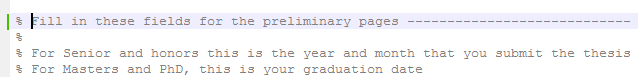
\includegraphics[width=5.0in]{preamble.png}
    \caption{Lines of \texttt{preambule.tex} after which the file should be modified.}
    \label{fig_preamble}
\end{figure}
\subsection{Frontmater: preamble.tex}\label{change_preamble}
In \texttt{preambule.tex} you have to modify everything that makes sense to be modified after the lines shown in Fig.~\ref{fig_preamble}. This includes your name, graduation month and year, your advisor, and etc. It also includes Acknowledgments and Abstract as well as the names of the members of your graduate committee except for the Committee Chair. If, besides the Committee Chair, you have three more committee members, then remove \% sign at the beginning of \texttt{MemberC\{\}} line, see Fig.~\ref{fig_members}.
\begin{figure}[ht!]
    \centering
    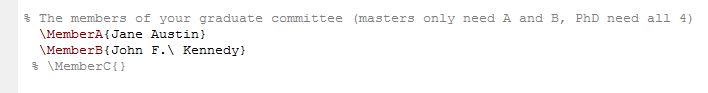
\includegraphics[width=5.0in]{members.png}
    \caption{Lines of \texttt{preambule.tex} for graduate committee members to be modified.}
    \label{fig_members}
\end{figure}
\begin{figure}[ht!]
    \centering
    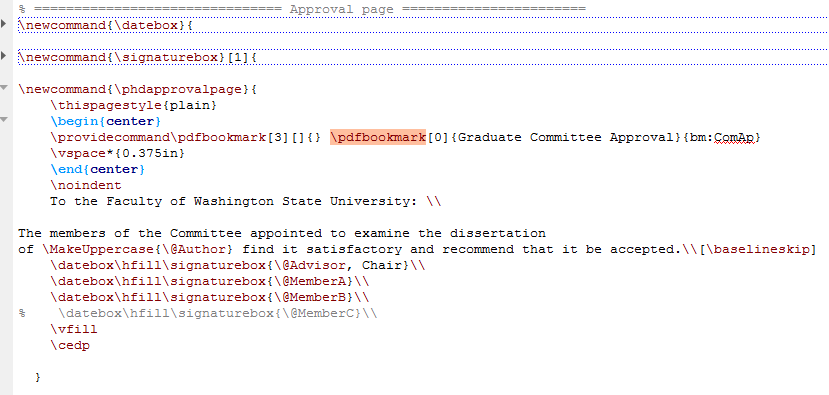
\includegraphics[width=5.0in]{wsu_class.png}
    \caption{Part of \texttt{WSUclass.cls} file to be modified.}
    \label{fig_wsu_class}
\end{figure}
\subsection{Supporting file: WSUclass.cls}\label{wsu_class}
After you are done modifying \texttt{preamble.tex}, you may need to do minor changes to \texttt{WSUclass.cls}. Figure~\ref{fig_wsu_class} shows the place where the file may need to be modified. The modification is required only if you have \texttt{MemberC\{\}} on your committee. If yes, then remove the \% sign to enable the line above the \texttt{\char`\\vfill}.
\subsection{Modifying dissertation text: maintext.tex}\label{change_maintext}
\texttt{maintext.tex} is where you put in your dissertation text. Modifying the file involves filling it with your content. Note that the file has structure - chapter, sections, subsections, and etc. Right now the file contains only a few examples showing how to format text, cite references, insert and cite figures, and etc.

{\em Remember}: while you modify the text in \texttt{maintext.tex}, you have to switch to \texttt{diss.tex} to build the document and view the changes. Every time you build the document, \texttt{diss.pdf} is saved to you working folder.
\subsection{Appendixes: app.tex}\label{change_app}
The file \texttt{app.tex} is where you put your appendixes in, see examples in the diss.pdf file.
\subsection{References: bib.bib}\label{change_refs}
Your bibliography is located in \texttt{bib.bib} file and managed by the \texttt{natbib} package in \texttt{diss.tex} file.
\subsubsection{Adding entries to your bibliography file}
Here is the easiest way I know how to add a new entry to \texttt{bib.bib} file. First, get the name of the article you need. Then search for it on Google Scholar. Once found, press 'Cite' link underneath it and choose 'BibTeX' in the pop-up window. A new tab will open. Copy the information from it into your bib file. That's it! 
\subsubsection{Citing references in the text}
Citation in LaTeX is straight forward. Suppose you have the following entry in the bib file:
\begin{verbatim}
@article{altschul1997gapped,
  title={Gapped BLAST and PSI-BLAST: a new generation of protein database search programs},
  author={Altschul, Stephen F and Madden, Thomas L and Sch{\"a}ffer, Alejandro A and Zhang, Jinghui and Zhang, Zheng and Miller, Webb and Lipman, David J},
  journal={Nucleic acids research},
  volume={25},
  number={17},
  pages={3389--3402},
  year={1997},
  publisher={Oxford Univ Press}
}
\end{verbatim}
\texttt{altschul1997gapped} is the label created for you. To cite this paper in the text, just type \texttt{\char`\\citep\{altschul1997gapped\}} and it will be cited appropriately. Also, see some examples in Chapter 1 in the \texttt{maintext.tex} file.

\section{Other Helpful Stuff}\label{sl:other}
\begin{figure}[ht!]
    \centering
    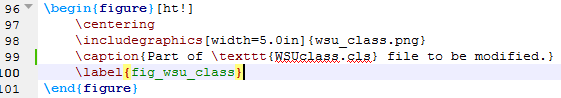
\includegraphics[width=4.0in]{fig_wsu_class.png}
    \caption{Code for Fig.~\ref{fig_wsu_class}.}
    \label{fig_wsu_class_code}
\end{figure}
\subsection{Referencing figures and tables in text}\label{refs_figs_tables}
Use a label for every figure and table you insert. Then you'll be able to reference them in the text automatically. For example, the code for the Figure~\ref{fig_wsu_class} has the label \texttt{fig\_wsu\_class} as shown in Fig.~\ref{fig_wsu_class_code}. To reference this figure in the text all you do is to call by its label like this \texttt{Fig.~\char`\\ref\{fig\_wsu\_class\}}. Figure numbering and order is kept automatically. The same rules apply to tables.
\section{ Disclaimer and Copyrights}
\subsection{History}
The LaTeX dissertation files came to me in early February of 2016 as I was working on my own dissertation. Their origins are obscure. The \texttt{WSUclass.cls} contained a reference to \texttt{BYUPhys} (later removed because it caused compiler error), but Brigham Young University, if what BYU stands for, does not have a physics department.
\subsection{For developers}
I modified the files to anonymize them and make them more automated as well as written this manual. I'm not a LaTeX guru and this is my only second time writing something in it. More things can be done to improve the files and this manual (as usual!). This is particularly true about the \texttt{WSUclass.cls}. It contains some known issues - such as, for example, adding an extra empty page - that need to be fixed. 
\subsection{Copyrights and Disclaimer}
This dissertation template is provided as-is, with no guarantees. You are free to modify, extend or distribute this code, as long as this copyright notice is included whole and unchanged.  

\begin{center}
{\huge Good Luck With Your Defense!}
\end{center}
\end{document}
